\documentclass[
   twoside,
   titlepage,
   numbers=noenddot,
   headinclude,
   footinclude=false, % no footer
   paper=a4,
   11pt,
]{scrreprt}

%%%%%%%%%%%%%%%%%%%%%%%%%%%%%%%
%% Custom adjustments %%%%%%%%%
%%%%%%%%%%%%%%%%%%%%%%%%%%%%%%%
\usepackage{float}
\usepackage{subcaption}
\usepackage{tabularx}
\usepackage{enumitem}
\usepackage{wrapfig}
\usepackage{caption}
\usepackage{placeins}
\usepackage{tablefootnote}
\usepackage{microtype}
\usepackage{subcaption}
\usepackage[dvipsnames,table,cymk]{xcolor}
\usepackage{multirow}
\usepackage{graphicx}
\usepackage{tikz}
\usepackage{pdfpages}

%% Pgfplots stuffs %%
\usepackage{pgfplots}
\pgfplotscreateplotcyclelist{color list}{%
   mark=*,black          \\%
   mark=*,RoyalBlue           \\%
   mark=*,webgreen         \\%
   mark=*,webbrown\\%
   mark=*,orange         \\%
   mark=*,blue           \\%
   mark=*,brown          \\%
   mark=*,cyan           \\%
   mark=*,green!70!black \\%
   mark=*,magenta        \\%
   mark=*,gray           \\%
}
\pgfplotscreateplotcyclelist{mylist}{
   mark=*,black        \\%
   mark=*,RoyalBlue          \\%
   mark=*,webgreen         \\%
   mark options=solid,mark=o,black,densely dashed\\%
   mark options=solid,mark=o,RoyalBlue,densely dashed\\%
   mark options=solid,mark=o,webgreen,densely dashed\\%
}
\pgfplotsset{
   grid style={dotted,gray},
   every axis/.append style={grid=both},
   every axis plot/.append style=
   {
      line width=1.2pt,
      mark options=solid,
   },
   cycle list name=color list,
   legend style={
      legend pos=south west,
      font=\tiny,
      legend style={row sep=-4pt},
      fill=white,
      fill opacity=0.6,
      draw opacity=1,
      text opacity=1,
   }
}

\usepackage[export]{adjustbox} % for max width in includegraphics

% Enable short captions in list of figures.
\usepackage{caption}
\usepackage{xparse}
\makeatletter
\let\latex@@caption\caption

\newif\ifallcaptionsshort% toggle switch
\allcaptionsshorttrue% Use the short ones

\RenewDocumentCommand{\caption}{+o+m}{%
  \def\@figcaptype{figure}
  \ifx\@captype\@figcaptype
  \ifallcaptionsshort
  \IfValueTF{#1}{%
    \latex@@caption[#1]{#2}%
  }{%
    \latex@@caption[#2]{#2}% No [#1] given, use the long caption then!
  }
  \else
  \latex@@caption[#2]{#2}%
  \fi
  \else
  \IfValueTF{#1}{%
    \latex@@caption[#1]{#2}%
  }{%
    \latex@@caption[#2]{#2}% No [#1] given, use the long caption then!
  }
  \fi
}
\makeatother

\usepgfplotslibrary{groupplots}
% compile plots to external file and then include -> faster compilation
\usepgfplotslibrary{external}
\tikzexternalize[prefix=gfx/autogen/,optimize command away=\includepdf]
\usepackage{pgfplotstable}
%% End Pgfplots stuffs %%

%% Other stuffs
\usepackage{graphicx}
\usepackage{IEEEtrantools}
\usepackage{tabularx}
\usepackage{mathtools}
\usepackage{stackengine}\stackMath % to use \stackgap for \underbrace spacing
\usepackage[
   german, % for correct hyphenation in german abstract
   english, % standard language
   american, % in order for the autorefnames to work (see below, could be changed)
]{babel}
\usepackage{setspace} % for adjustment of line spacing
\usepackage[lined,boxed,linesnumbered]{algorithm2e}

% \expandafter\def\csname ver@subfig.sty\endcsname{} % for subcaption or
% something
\bibliographystyle{apa}

\newcommand{\mbf}[1]{\mathbf{#1}} % shortcut for vector notation

\newcommand{\bflabel}{\aclabelfont} % without this, compile error

\usepackage{chngcntr} % defines \counterwithin
\counterwithin{figure}{chapter} % number figures as chaptno.figno
\counterwithin{equation}{chapter} % number equations as chaptno.eqno

\SetAlCapSkip{1ex} % algorithm2e distance between caption an algorithm
\newcommand{\sub}[2]{#1_{\text{#2}}}
\let\originaleqref\ref
\makeatletter
\renewcommand{\eqref}[1]{%
   \begingroup%
   \let\ref\@refstar%
   \hyperref[#1]{%
      equation%
      ~\originaleqref{#1}%
   }%
   \endgroup
}
\makeatother
\DeclareMathOperator{\atan2}{atan2}
%%%%%%%%%%%%%%%%%%%%%%%%%%%%%%%
%% End Custom adjustments %%%%%
%%%%%%%%%%%%%%%%%%%%%%%%%%%%%%%


% ****************************************************************************************************
% 1. Configure classicthesis for your needs here, e.g., remove "drafting" below
% in order to deactivate the time-stamp on the pages
% ****************************************************************************************************
\PassOptionsToPackage{
   eulerchapternumbers,
   listings,
   pdfspacing,
   floatperchapter,
   %linedheaders,
   beramono,
   eulermath,
   parts,
   dottedtoc
}{classicthesis}
% ********************************************************************
% Available options for classicthesis.sty
% (see ClassicThesis.pdf for more information):
% drafting
% parts nochapters linedheaders
% eulerchapternumbers beramono eulermath pdfspacing minionprospacing
% tocaligned dottedtoc manychapters
% listings floatperchapter subfig
% ********************************************************************


% ********************************************************************
% Triggers for this config
% ********************************************************************
\usepackage{ifthen}
\newboolean{enable-backrefs} % enable backrefs in the bibliography
\setboolean{enable-backrefs}{true} % true false
% ****************************************************************************************************

% Custom colour definitions
\definecolor{verylightblue}{RGB}{243, 243, 250}
\definecolor{verydarkblue}{RGB}{37, 65, 103}
\definecolor{reddish}{RGB}{238, 86, 121}
\definecolor{yellowish}{RGB}{217, 216, 116}
\definecolor{mediumlightblue}{RGB}{157, 176, 191}


% ****************************************************************************************************
% 2. Personal data and user ad-hoc commands
% ****************************************************************************************************
\newcommand{\myTitle}{Live Introspection for Neural Network Training}
\newcommand{\myName}{Rasmus Diederichsen\xspace}
\newcommand{\myFirstSupervisor}{Prof. Dr. Oliver Vornberger\xspace}
\newcommand{\mySecondSupervisor}{Dr. Ulf Krumnack\xspace}
\newcommand{\myProjectSupervisor}{Anders Arpteg, PhD\xspace}
\newcommand{\myUni}{Osnabrück University\xspace}

% ********************************************************************
% Setup, finetuning, and useful commands
% ********************************************************************
\newcounter{dummy} % necessary for correct hyperlinks (to index, bib, etc.)
\newlength{\abcd} % for ab..z string length calculation
\providecommand{\mLyX}{L\kern-.1667em\lower.25em\hbox{Y}\kern-.125emX\@}
% ****************************************************************************************************


% ****************************************************************************************************
% 3. Loading some handy packages
% ****************************************************************************************************
% ********************************************************************
% Packages with options that might require adjustments
% ********************************************************************
\PassOptionsToPackage{utf8}{inputenc}	% latin9 (ISO-8859-9) = latin1+"Euro sign"
\usepackage{inputenc}

%\PassOptionsToPackage{ngerman,american}{babel}   % change this to your language(s)
% Spanish languages need extra options in order to work with this template
%\PassOptionsToPackage{spanish,es-lcroman}{babel}
\usepackage[english]{babel}

\PassOptionsToPackage{authoryear,round,colon}{natbib}
\usepackage{natbib}

\PassOptionsToPackage{fleqn}{amsmath}		% math environments and more by the AMS
\usepackage{amsmath}
\DeclareMathOperator{\Span}{span}

% ********************************************************************
% General useful packages
% ********************************************************************
\PassOptionsToPackage{T1}{fontenc} % T2A for cyrillics
\usepackage{fontenc}
\usepackage{textcomp} % fix warning with missing font shapes
\usepackage{scrhack} % fix warnings when using KOMA with listings package
\usepackage{xspace} % to get the spacing after macros right
\usepackage{mparhack} % get marginpar right
\PassOptionsToPackage{printonlyused,smaller}{acronym}
\usepackage{acronym} % nice macros for handling all acronyms in the thesis
%\renewcommand*{\acsfont}[1]{\textssc{#1}} % for MinionPro
\renewcommand{\bflabel}[1]{{#1}\hfill} % fix the list of acronyms
% ****************************************************************************************************


% ****************************************************************************************************
% 4. Setup floats: tables, (sub)figures, and captions
% ****************************************************************************************************
\usepackage{tabularx} % better tables
\setlength{\extrarowheight}{3pt} % increase table row height
\newcommand{\tableheadline}[1]{\multicolumn{1}{c}{\spacedlowsmallcaps{#1}}}
\newcommand{\myfloatalign}{\centering} % to be used with each float for alignment
\usepackage{caption}
\captionsetup{format=hang,font=small}
% ****************************************************************************************************


% ****************************************************************************************************
% 5. Setup code listings
% ****************************************************************************************************
\usepackage{listings}
%\lstset{emph={trueIndex,root},emphstyle=\color{BlueViolet}}%\underbar} % for special keywords
\lstset{language=Python,
    otherkeywords={self,__init__},
    deletekeywords={sum},
    captionpos=b,
    basicstyle=\footnotesize\ttfamily,
    keywordstyle=\color{reddish},%\bfseries,
    % identifierstyle=\color{NavyBlue},
    commentstyle=\color{mediumlightblue},
    stringstyle=\color{verydarkblue},
    numbers=none,%left,%
    numberstyle=\scriptsize,%\tiny
    stepnumber=5,
    numbersep=8pt,
    showstringspaces=false,
    breaklines=true,
    frameround=ffff,
    frame=single,
    rulecolor=\color{black}
}
% ****************************************************************************************************


% ****************************************************************************************************
% 6. PDFLaTeX, hyperreferences and citation backreferences
% ****************************************************************************************************
% ********************************************************************
% Using PDFLaTeX
% ********************************************************************
\PassOptionsToPackage{pdftex, pdfpagelabels}{hyperref}
\usepackage{hyperref}  % backref linktocpage pagebackref
\pdfcompresslevel=9
\pdfadjustspacing=1
\PassOptionsToPackage{pdftex}{graphicx}


% ********************************************************************
% Setup the style of the backrefs from the bibliography
% (translate the options to any language you use)
% ********************************************************************
\newcommand{\backrefnotcitedstring}{\relax}%(Not cited.)
\newcommand{\backrefcitedsinglestring}[1]{(Cited on page~#1.)}
\newcommand{\backrefcitedmultistring}[1]{(Cited on pages~#1.)}
\ifthenelse{\boolean{enable-backrefs}}%
{%
   \PassOptionsToPackage{hyperpageref}{backref}
   \usepackage{backref} % to be loaded after hyperref package
   \renewcommand{\backreftwosep}{ and~} % separate 2 pages
   \renewcommand{\backreflastsep}{, and~} % separate last of longer list
   \renewcommand*{\backref}[1]{}  % disable standard
   \renewcommand*{\backrefalt}[4]{% detailed backref
      \ifcase #1 %
      \backrefnotcitedstring%
      \or%
      \backrefcitedsinglestring{#2}%
      \else%
      \backrefcitedmultistring{#2}%
   \fi}%
}{\relax}

% ********************************************************************
% Hyperreferences
% ********************************************************************
\hypersetup{%
    % draft,	% = no hyperlinking at all (useful in b/w printouts)
    linktocpage=false, pdfstartpage=3, pdfstartview=FitV,%
    % uncomment the following line if you want to have black links (e.g., for printing)
    %colorlinks=false, linktocpage=false, pdfborder={0 0 0}, pdfstartpage=3, pdfstartview=FitV,%
    breaklinks=true, pdfpagemode=UseNone, pageanchor=true, pdfpagemode=UseOutlines,%
    plainpages=false, bookmarksnumbered, bookmarksopen=true, bookmarksopenlevel=1,%
    hypertexnames=true, pdfhighlight=/O,%nesting=true,%frenchlinks,%
    pdftitle={\myTitle},%
    pdfauthor={\textcopyright\ \myName, \myUni},%
    pdfsubject={},%
    pdfkeywords={},%
    pdfcreator={pdfLaTeX},%
    pdfproducer={LaTeX with hyperref and classicthesis}%,
    breaklinks=true,
    hyperfootnotes=true,
    bookmarks=true,
    pdfauthor=\myName,
    pdftitle=\myTitle,
    citecolor=verydarkblue,
    urlcolor=reddish,
    linkcolor=verydarkblue
    colorlinks=false,   % #wtflatex: This doesn't do anything, the only way to
                        % disable colors is to remove them altogether with the drafting option
}

% ********************************************************************
% Setup autoreferences
% ********************************************************************
% There are some issues regarding autorefnames
% http://www.ureader.de/msg/136221647.aspx
% http://www.tex.ac.uk/cgi-bin/texfaq2html?label=latexwords
% you have to redefine the makros for the
% language you use, e.g., american, ngerman
% (as chosen when loading babel/AtBeginDocument)
% ********************************************************************
\makeatletter
\@ifpackageloaded{babel}%
{%
   \addto\extrasamerican{%
      \renewcommand*{\algorithmautorefname}{Algorithm}%
      \renewcommand*{\figureautorefname}{Figure}%
      \renewcommand*{\tableautorefname}{Table}%
      \renewcommand*{\partautorefname}{Part}%
      \renewcommand*{\chapterautorefname}{Chapter}%
      \renewcommand*{\sectionautorefname}{Section}%
      \renewcommand*{\subsectionautorefname}{Subsection}%
      \renewcommand*{\subsubsectionautorefname}{Subsubsection}%
   }%
   \addto\extrasngerman{%
      \renewcommand*{\paragraphautorefname}{Absatz}%
      \renewcommand*{\subparagraphautorefname}{Unterabsatz}%
      \renewcommand*{\footnoteautorefname}{Fu\"snote}%
      \renewcommand*{\FancyVerbLineautorefname}{Zeile}%
      \renewcommand*{\theoremautorefname}{Theorem}%
      \renewcommand*{\appendixautorefname}{Anhang}%
      \renewcommand*{\equationautorefname}{Gleichung}%
   \renewcommand*{\itemautorefname}{Punkt}%
   }%
   % Fix to getting autorefs for subfigures right (thanks to Belinda Vogt for changing the definition)
   \providecommand{\subfigureautorefname}{\figureautorefname}%
}{\relax}
\makeatother


% ****************************************************************************************************
% 7. Last calls before the bar closes
% ****************************************************************************************************
% ********************************************************************
% Development Stuff
% ********************************************************************
\listfiles
%\PassOptionsToPackage{l2tabu,orthodox,abort}{nag}
%	\usepackage{nag}
%\PassOptionsToPackage{warning, all}{onlyamsmath}
%	\usepackage{onlyamsmath}

% ********************************************************************
% Last, but not least...
% ********************************************************************
\usepackage{classicthesis}
% ****************************************************************************************************


% ****************************************************************************************************
% 8. Further adjustments (experimental)
% ****************************************************************************************************
% ********************************************************************
% Changing the text area
% ********************************************************************
%\linespread{1.05} % a bit more for Palatino
%\areaset[current]{312pt}{761pt} % 686 (factor 2.2) + 33 head + 42 head \the\footskip
%\setlength{\marginparwidth}{7em}%
%\setlength{\marginparsep}{2em}%

% ********************************************************************
% Using different fonts
% ********************************************************************
% \usepackage[oldstylenums]{kpfonts} % oldstyle notextcomp
%\usepackage[osf]{libertine}
% \usepackage{hfoldsty} % Computer Modern with osf
%\usepackage[light,condensed,math]{iwona}
%\renewcommand{\sfdefault}{iwona}
%\usepackage{lmodern} % <-- no osf support :-(
%\usepackage[urw-garamond]{mathdesign} %<-- no osf support :-(
% ****************************************************************************************************

%% Should be loaded after classicthesis
\usepackage{ebgaramond}
\usepackage[scale=0.9]{sourcecodepro}

\usepackage[noabbrev, nameinlink]{cleveref}

% https://tex.stackexchange.com/a/63242/31250
\usepackage{xhfill}
\newcommand{\ditto}[1][.4pt]{\xrfill{#1}~\textquotedbl~\xrfill{#1}}
 % all custom classicthesis config stuff
% \renewcommand{\bibsection}{\chapter{\bibname}} % this gives the bib entry the
% same style as the other toc lines, but also makes the bib a true appendix,
% which is unwanted

\begin{document}
% \onehalfspacing
\raggedbottom
\pagenumbering{roman}
\pagestyle{plain}

%*******************************************************
% Frontmatter
%*******************************************************
\thispagestyle{empty}


\includepdf{FrontBackmatter/Titlepage.pdf}

\cleardoublepage
\chapter*{Abstract}

Artificial neural networks have become the prevalent model class for many
machine learning tasks, including image classification, segmentation, video and
audio analysis, or time series prediction. With ever increasing computational
resources and advances in programming infrastructure, the size of model we can
train also increases. Nevertheless, it is not uncommon for training to take days
or weeks, even on potent hardware. While there are many obvious causes -- e.g.
inherent difficulty to parallelize training with the most successful algorithms
-- tere may still be inefficiencies due to our incomplete knowledge of training
dynamics which is compensated for by expensive parameter search.

The pragmatic approach to opening the black box of deep learning is
through experimentation and observation. Experiments are being performed to
obtain insights into the training process and said insights can then be used to
guide the training.  The speed and ease at which experiments can be performed is
tied to the availability of tooling for the experimentor.

In this thesis, a software library is presented which facilitates both
experimenting on metrics which can guide and ultimately accelerate the learning
process and monitoring these metrics in practice. The library is then used to
investigate a selection of metrics in order to find out if heretofore unknown
signals can be extractd for informing parameter choices during training. Also,
the library is used for validating known or claimed results, highlighting its
usefulness for deep learning research.

\chapter*{Zusammenfassung}

\begin{otherlanguage}{german}

    Künstliche neuronale Netze sind inzwischen die populärste Art von Modell für
    viele Anwendungen im maschinellen Lernen, z.B. Bildklassifikation,
    Segmentierung oder Video- und Audioanalyse sowie Zeitreihenvorhersage.  Mit
    immer zunehmenden Ressourcen und Fortschritten in verfügbarer Software
    steigt auch die Größe der Trainierbaren Modelle. Dennoch sind
    Trainingszeiten von Tagen und Wochen -- selbst auf potenter Hardware --
    nicht ungewöhnlich.

    Es gibt naheliegende Ursachen -- z.B. die Schwierigkeit, das Training zu
    parallelisieren aufgrund der eingesetzten Optimierungsalgorithmen -- jedoch
    möglicherweise auch weninger offensichtliche Verluste in der Art und Weise,
    wie Modelle normalerweise trainiert werden.

    Während der praktische Erfolg tiefer neuronaler Netze rapide war, konnte die
    theoretische Erschließung nicht Schritt halten, und viele fortschrittliche
    Ideen sind mehr von Intuition und Experimenten gestützt als von rigorosen
    Formalismen.  Für die meisten erfolgreichen Ideen haben wir folglich kein
    klares Verständnis dafür, warum sie in der Praxis gut funktionieren.

    Diese Kluft zwischen Praxis und Theorie ist auch ursächlich dafür, dass
    Deep-Learning-Applikationen mehr als Kunst denn als Wissenschaft gelten.
    Anders als in der traditionellen Softwareentwicklung, die auf Jahrzenten der
    Forschung in Ingenieurswissenschaften, Mathematik und theoretischer
    Informatik basiert, gibt es im maschinellen Lernen oft keinen definitiven
    Ansatz, um ein konkretes Problem zu lösen. Des Weiteren sind die verfügbaren
    Debugging-Werkzeuge in jeder Schicht der Softwareentwicklung denen des Deep
    Learning bei weitem überlegen. Einfache Fragen wie ``Lernt das Modell das,
    was ich möchte?'' sind bislang nicht zu beantworten. Wir können hier also
    eine Notwendigkeit für mehr nützliche Tools für Anwender konstatieren.

    Der Standardweg, eine gute Parameterwahl für das Modell zu treffen, ist
    Trial-and-Error oder etwas intelligentere Variationen davon. Der
    Rechenaufwand für das Training großer Modelle verhindert schnelles
    Experimentieren und schlägt sich häufig auch in finanziellen Kosten für die
    nötige Rechenleistung nieder.  Frühzeitig Sackgassen zu identifizieren oder
    Zeitpunkte, an denen man bestimmte Parameter ändern sollte, könnten daher
    große Ersparnisse bedeuten.

    Diese Arbeit stellt zum Einen eine Softwarebibliothek vor, die im Debugging
    von Deep-Learning-Anwendungen hilft und das Experimentieren erleichtert. Zum
    Anderen wird dieses Werkzeug benutzt, um experimentell festzustellen, ob aus
    dem Trainingsprozess Signale extrahiert werden können, die Aufschluss über
    die Wahl von Parametern geben, während das Training läuft.

\end{otherlanguage}


\pagestyle{scrheadings}

%*******************************************************
% Mainmatter
%*******************************************************
% use \cleardoublepage here to avoid problems with pdfbookmark
\cleardoublepage

\tableofcontents

\listoftables

\listoffigures

% \newpage % #wtflatex Funnily, if I leave this out, the below statement applies
% to the page this list ist typeset on. This is ridiculous, how am I the first
% one to see this?

\pagenumbering{arabic}

\chapter{Introduction}\label{sec:introduction}

While the success of deep learning models has been rapid, the theoretical
justification for most game-changing ideas as well as the general principles of
deep learning has not kept pace (for more information, see \cite{arora2018}).
This means that for many successful techniques, we have no clear understanding
why they work so well in practice.

This explanatory gap is also a reason why developing deep learning applications
is considered more of an art than a science. In contrast to traditional
programming, which builds on decades of research and development in electrical
engineering, logic, mathematics and theoretical computer science, there's rarely
one definitive way to solve a certain problem in deep learning.  Additionally,
the quality of debugging tools available to a programmer on every level of
abstraction far exceeds what we currently have for differentiable programming.
Simple questions like ``Does my model learn what I want it to learn?'' are not
answerable at this point.  We can thus identify a need to supply more useful
tooling for deep learning researchers and practitioners.  A standard approach to
choosing a parametrisation remains trial-and-error, or only somewhat more
sophisticated ways to run and test.  The computational cost of training large
models prohibits quick experimentation and often translates into monetary costs
as well.  Identifying dead ends early or points in training at which to tweak
certain parameters could thus provide large savings in time and money, besides
enabling a more thorough understanding of what is going on inside the pile of
linear algebra that is a deep learning model.

This thesis addresses the above in two ways: A software library aiding in deep
learning debugging and experimentation is designed, implemented and documented. The same
library is then used to investigate experimentally whether unexplored
metrics can be devised for optimising parameters of the training process while it is running.

This thesis is concerned with \emph{deep} neural networks, meaning
architectures consisting of many layers. Typically, the number of units
in such a model and thus the number of tunable parameters
(\(n_{weights\_per\_neuron} \times n_{neurons}\)) exceeds the number of
training examples. Training such large networks thus involves iterating
over the dataset many times which incurs a high computational cost due
to the massive number of matrix operations involved. Speeding up the
training is thus one of the primary endeavours in deep learning
research. An overview of the workings of a neural network is given in
\cref{sec:anns}.

\hypertarget{sec:anns}{%
\section{Artificial Neural Networks}\label{sec:anns}}

The artificial neural network is a class of machine learning model which can be
used for regression, classification, generation and a host of other tasks.  At
its core, neuronal models are simply conceptualised as an arrangement of units
which receive numerical inputs, compute a weighted sum and thus produce an output
activation. The ideas date back at least to Hebbian learning (a single neuron)
in the 1940s, and were developed into the Perceptron model by
\citet{Rosenblatt58theperceptron}. With the introduction of the backpropagation
algorithm \citep{werbos1975beyond} and increasing availability of computing
power, this began to change, but more easily trainable models like Support
Vector machines eclipsed neural nets for most applications.  Architectural
advances, such as the convolutional neural networks in the late 1980s
\citep{LeCun:1989:BAH:1351079.1351090} and the advent of GPU-accelerated neural
network implementations (pioneered in \cite{Ciresan11flexible}) -- as well as
subsequently, gpu-accelerated linear algebra libraries with automatic
differentiation -- finally made neural networks the workhorse for many AI
applications today.

A neural network consists of at least one input layer, \(0-n\)
intermediate layers and at least one output layer. Data is processed in
numerical form by multiplying it with the input layer's weights, mapping
each product with the input layer's activation function and then
propagating the resulting activations through subsequent layers in the
same fashion. \Cref{fig:neuralnet} gives a graphical representation of a
multi-layer feedforward network.

\begin{figure}
    \hypertarget{fig:neuralnet}{%
        \centering
        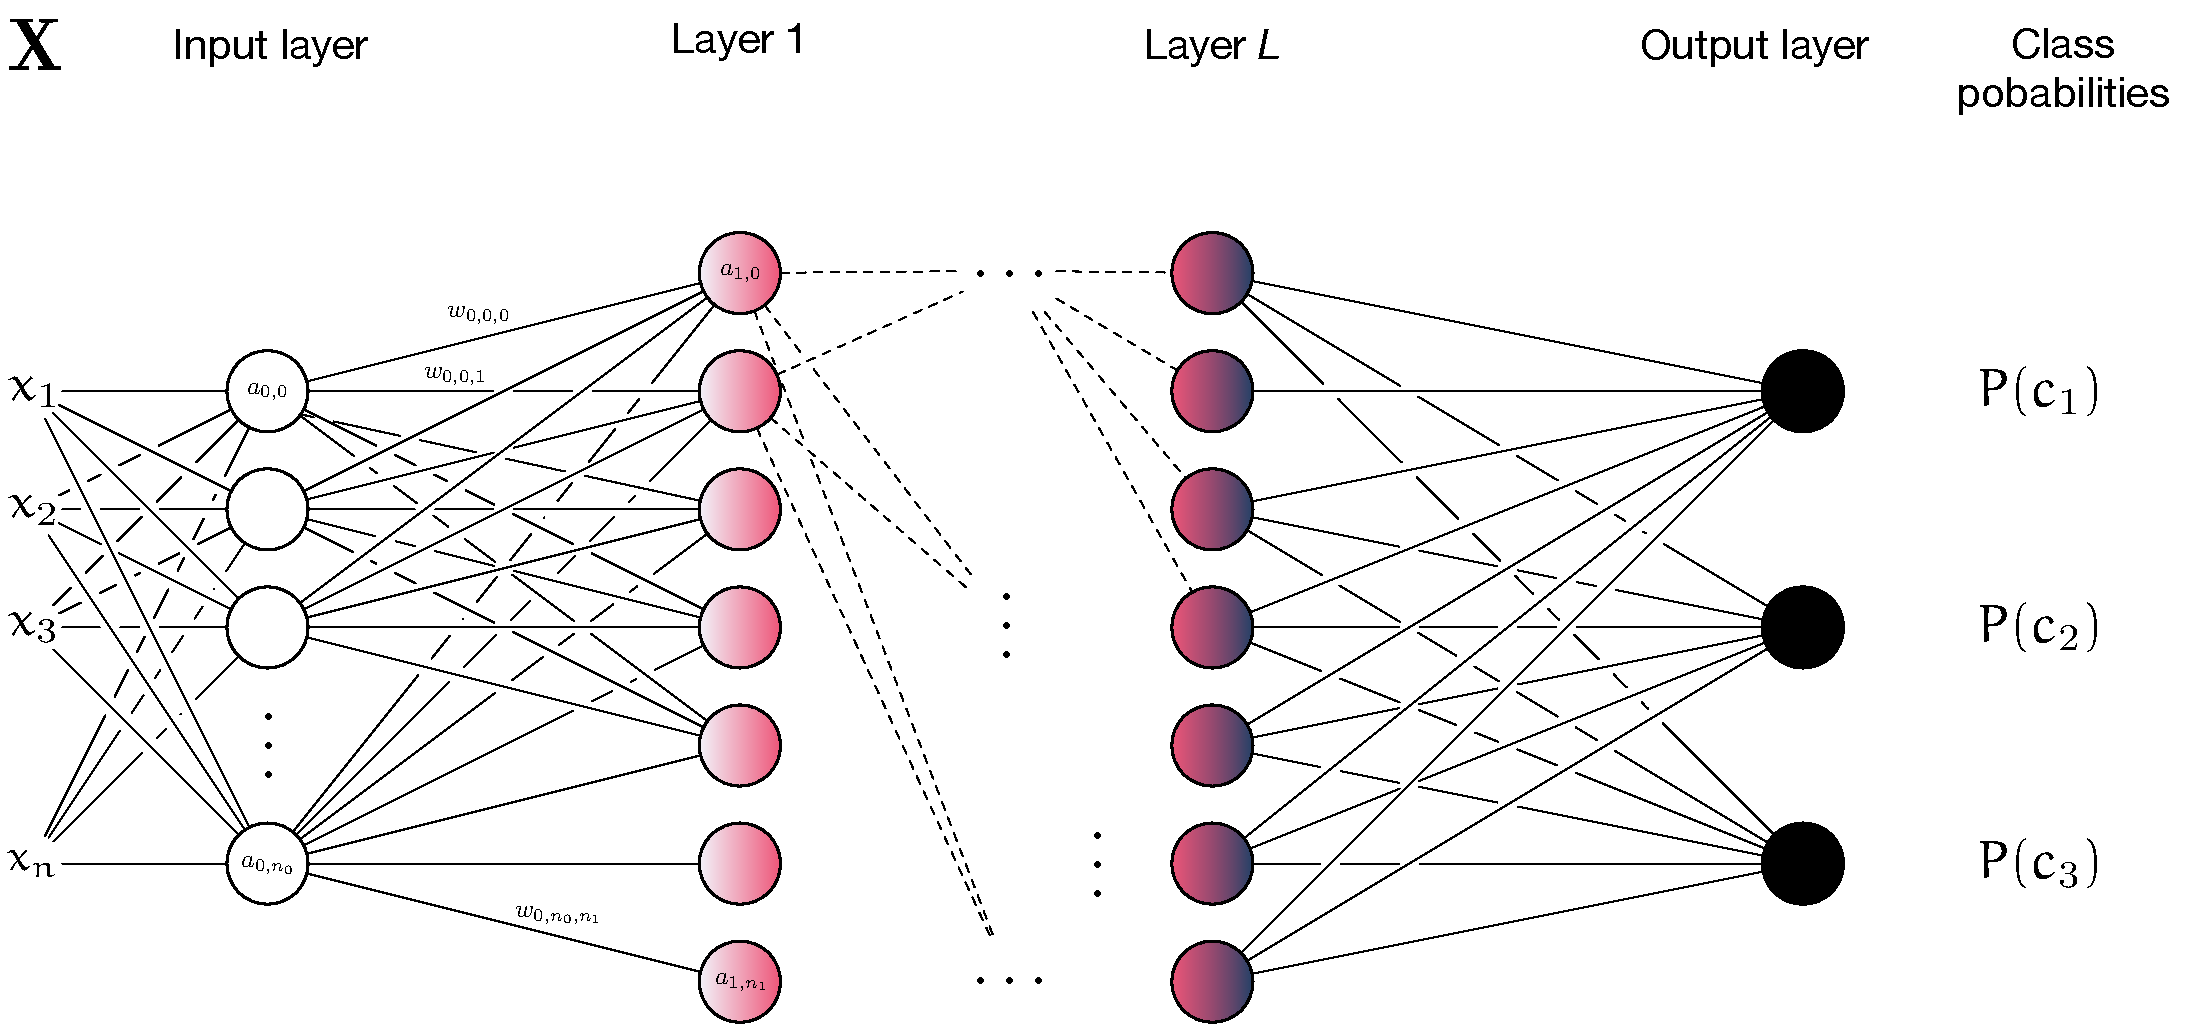
\includegraphics[max width=\textwidth]{gfx/diagrams/neural_network/neural_net.pdf}
        \caption[Schema of a multi-layer neural network]{Schema of a multi-layer neural network. \(\mathbf{x}_i\) are
            the input values, \(a_{l_n,i}\) the \(i\)-th activation in layer \(l_n\)
            and \(w_{l_n,i,j}\) the weight between the \(i\)-th unit in layer
        \(l_n\) and the \(j\)-th unit in layer \(l_{n+1}\)}\label{fig:neuralnet}
    }
\end{figure}

Training a neural network simply involves a loss function measuring the distance
of the networks output to the desired output and differentiating it with respect
to the model parameters. The backpropagation algorithm provides an efficient way
of computing all the partial derivatives of the loss with respect to each
parameter (network weight). Parameters are usually updated with some form of the
gradient descent optimisation algorithm. An introduction to the mathematics of
deep neural networks is deferred to
\cref{sec:review_stochastic_gradient_descent}.

\hypertarget{sec:thesis-goals}{%
\section{Goals of this Thesis}\label{sec:thesis-goals}}

The objective of this work is twofold:

\begin{enumerate}
    \item
        Create a software library that enables easy and reusable
        implementation of training metrics and abstracts away the concrete model
        architecture
    \item
        Perform experiments on common datasets to investigate whether common
        problems in neural network training can be detected by the use of
        appropriate metrics. Issues which could be investigated include, but are
        not limited to
        \begin{itemize}
            \item
                inappropriate learning rate
            \item
                layer/model saturation
            \item
                bad initialisations
            \item
                inappropriate network architecture
            \item
                bad generalisation/overfitting
            \item
                susceptibility to adversarial attacks
        \end{itemize}
\end{enumerate}

\hypertarget{sec:motivation}{%
\section{Motivation}\label{sec:motivation}}

In contrast to classical machine learning models, training deep neural networks
requires navigating a huge parameter space. While most non-neural regression or
classification algorithms only require specification of a parameter set up-front
and often no more than a few, some parameters can (and should) be varied over
training time for neural networks. Looking at the popular scikit-learn library \citep{scikit-learn},
it can be seen that traditional methods such as SVMs, Gaussian Processes,
Decision Trees or Gradient Boosting typically require less than $10$
hyperparameters\footnote{A look through
\href{http://scikit-learn.org/stable/supervised_learning.html\#supervised-learning}{scikit-learn}s
selection of regressors and classifiers shows most classes require between 5 and
10 parameters.}.

In neural networks the parameter space can have arbitrarily many dimensions when
factoring in the fact that some parameters can change over time, such as

\begin{itemize}
    \item
        learning rate (can be annealed)
    \item
        batch size\footnote{It is not usual to change the batch size during
            training, but it can have an effect similar annealing the learning
        rate (see \cite{DBLP:journals/corr/abs-1711-00489})}
    \item
        trainability of layers (not all layers need to be trained throughout the
        entire training)
\end{itemize}

Other parameters that need to be set initially are

\begin{itemize}
    \item
        Network architecture (how many layers, how many units per layer,
        what kind of layers)
    \item
        nonlinearity function for each layer
    \item
        loss function
    \item
        optimisation algorithm
    \item
        initial learning rate
    \item
        momentum of the weight updates
    \item
        weight decay
    \item
        Regularisation methods for the weights
\end{itemize}

This makes finding an optimal training regimen very hard, particularly since
training deep neural networks for realistic problems can take much longer than
traditional methods, meaning cross-validating different models can be
prohibitively expensive. It is therefore desirable to notice dead ends early
during training, or be able to tweak parameters in such a way as to maximise
convergence speed.

This thesis work is motivated by the scarcity of useful tools to debug and
monitor deep learning training. \citet{arpteg2018software} discuss several
challenges arising in the context of engineering larger-scale machine learning
software and note that a lack of useful debugging tools can lead to a lot of
wasted time and money in diagnosing problematic behaviour of a neural network.

Without years of training and a lot of
mathematical intuition and expertise, it is often very hard to figure out why a
network is not learning or how to ensure timely convergence.  And even with this
expertise, visualisations or metrics need to be implemented over and over again
because common tools do not abstract from the concrete model architecture.
Providing easy-to-use tooling and live insights also has the side-effect of
democratising access to machine learning software. Ideally, the metrics created
with the help of this work would enable non-experts to better understand their
models and reduce the dependence on rare machine learning expertise. While this
goal will likely not be achieved by this work alone, steps in the general
direction are needed for disseminating AI advances throughout the industry, and
counteract the tendency of large companies to reap the majority of the benefits
brought about by deep learning.

There exist a some of monitoring tools (see \cref{sec:existing-apps}), but they
are mostly low-level tools which provide visualisation primitives (drawing and
interacting with graphs). They may enable visualisation of certain network
metrics on top of the primitives, but there is no native support for a concept
such as \emph{Maximum singular value of the weight matrix} which can be simply
applied automatically to all layers.

In contrast, the library developed in this work is geared towards modularising
introspection metrics in such a way that they are usable for any kind of model,
without modifications to the model code. The secondary purpose of the library is
the enablement to quickly iterate on hypothesised metrics extracted from the
training in order to diagnose problems such as those outlined in
\cref{sec:thesis-goals}. Most deep learning research involves experiments on a
variety of architectures, datasets, and hyperparameter sets in order to validate
an idea. All of these experiments must be implemented, which can easily lead to
haphazard duplication of code for all the different settings, or creation of
ad-hoc libraries that are only used in this specific work. Thus, a lot of effort
is wasted due to the lack of more general tools and the fact that code produced
for research often is not made public, or would require significant effort to
generalise to other problems.

As such, the library shall not only be useful to end users who will make use of
established metrics and thus save time in their model training, but also to
researchers and the author of this thesis in evaluating hypotheses about
training metrics.

In summary, this library is supposed to be both a developer tool, reducing
implementation effort, decreasing opacity of the training process and a research tool for
abstracting away some of the nuisances of machine learning experimentation and
simplifying experiments for live metrics in neural networks.

\hypertarget{sec:existing-apps}{%
\section{Existing Applications}\label{sec:existing-apps}}

There exist a variety of libraries for machine learning visualisation which we
will briefly survey in this section.

\hypertarget{tensorboard}{%
\subsection*{TensorBoard}\label{tensorboard}}

TensorBoard is a visulisation toolkit originally developed for the TensorFlow
\citep{tensorflow2015-whitepaper} deep learning framework. It is composed of a
Python library for exporting data from the training process and a web server
which reads the serialised data and displays it in the browser. The server can
be used independently from TensorFlow, provided the data is serialised in the
appropriate format. This enables, e.g., a PyTorch port, termed TensorBoardX.

For exporting data during training, the developer adds operations to the
graph which write scalars, histograms, audio, or other data
asynchronously to disk. This data can then be displayed in approximately
real-time in the web browser. Besides scalar-valued functions, which
could be e.g.~the loss curve or accuracy measure, TensorBoard supports
histograms, audio, and embedding data natively. However, concrete
instances of these classes of training artifact must be defined by the
user and can only be reused if the developer creates a separate library
for the computations involved. TensorBoard or TensorFlow also have no built-in
way of intelligently discovering the model structure to automatically add
visualisations of every layer with a higher-level API.

New kinds of visualisations can be added with plugins, which require not
only writing the Python code exporting the data and for serving it from
the web server, but also JavaScript for actually displaying it (the
Polymer library is used for this\footnote{\url{https://www.polymer-project.org/}}).

An attempt to abstract over the programming language for talking to
the server is \href{https://github.com/torrvision/crayon}{Crayon} which
so far supports Python and Lua.

In summary, TensorBoard is a possible backend for the library developed here,
but operates at a lower level of abstraction.

\hypertarget{visdom}{%
\subsection*{Visdom}\label{visdom}}

Visdom by Facebook Research fulfills more or less the same purpose as
TensorBoard, but supports Numpy and Lua Torch. In contrast to
TensorBoard, Visdom includes more features for organising the display of
many visualisations at once. Still, the framework is mostly geared
towards improving workflows for data scientists, and is not concerned
with providing useful metrics out-of-the-box.

\hypertarget{others}{%
\subsection*{Others}\label{others}}

There are other tools such as \href{http://yosinski.com/deepvis}{DeepVis} for
offline introspection by e.g.  visualising learned features, which offer
insights into the training after the fact, but do not help guiding the training
process while it is running.

General-Purpose plotting libraries such as MatplotLib fall into the same
category as TensorBoard -- they offer primitives but there are no dedicated
extensions to work with neural networks.


\hypertarget{ikkuna}{%
\chapter{Ikkuna}\label{ikkuna}}

Ikkuna is the Python library developed for this thesis. It targets
Python 3.6 and was designed with the following goals in mind:

\begin{enumerate}
    \item
        Ease of use. Minimal configuration, maximum rewards.
    \item
        Flexible and all-encompassing API enabling creating arbitrary metrics
        which act on training artifacts
    \item
        Metrics shall be agnostic of model code.
    \item
        Plugin architecture so metrics written once can be used for any kind
        of model
    \item
        Framework agnosticism. Ideally, the library would support every deep
        learning framework through an extensible abstraction layer.
\end{enumerate}

What it provides over the aforementioned tools is that it enables
working at a higher level of abstraction, liberating the developer from
having to repeat herself, exchanging visualizations and metrics and
reduce the friction between development and debugging. This chapters gives a
high-level overview of the library components and elaborates on the design
decisions made during the creation. Throughout the chapters, UML class and
package diagrams will serve as a mental map for the reader. For brevity, not all
parts of the library are diagrammed down to the same level of detail.

\hypertarget{design-principles}{%
\section{Design Principles}\label{design-principles}}

Of the aforementioned goals, all except one have been accomplished. The
objective of making the library agnostic to the deep learning framework
being used (TensorFlow, PyTorch, PyCaffe, Chainer, etc.) has been
neglected for practical reasons. Enabling this kind of support is beyond
the scope of this thesis and only requires the implementation of a
software layer which offers framework-agnostic access to network
modules, activations, gradients and all the other necessary information.
While this is certainly possible and useful, the PyTorch framework has
been chosen for this work to create a proof of the concept. The choice is
motivated in \cref{sec:dl-frameworks}.

The overarching architecture of this software must lend itself to this
agnosticity goal, however. As such, a very loose coupling between model code,
metric computation and visualizations is desired. Not only will this aid in
extending the library to different deep learning frameworks, but it is also a
prerequisite for allowing for modular, self-contained visualizations or metrics
which can be installed and used separately and independently of specific model
code. The Publisher-Subscriber design pattern has been chosen for these reasons
(\cref{sec:pubsub}).

\hypertarget{sec:dl-frameworks}{%
\section{Deep Learning frameworks}\label{sec:dl-frameworks}}

The currently available deep learning libraries can be located on a spectrum
between define-by-run and define-and-run.  The first extreme would be a
framework such as PyTorch \citep{paszke2017automatic} or Chainer
\citep{tokui2015chainer} , where there exist no two distinct execution phases --
just like in an ordinary matrix library like NumPy, each statement immediately
returns or operates on an actual value. By contrast, graph-based frameworks like
TensorFlow\footnote{Since version 1.4, TensorFlow gravitates toward
    define-by-run through the introduction of \emph{eager execution}, which
becomes the default mode in version 2.0. Graph-based execution is still
available, but not the default any longer.} require specifying the model graph
in a domain-specific language (TensorFlow has Python, Java and C++ APIs, Caffe
uses Prototxt files), compile it to a different representation and the the model
is run and trained in a second phase. While this enables graph-based
optimizations, the main downsides are that

\begin{itemize}
    \item
        control flow cannot use the host language features, but must be done
        with the API used for defining models. Instead of
        \begin{lstlisting}[language=Python, label=lst:whilepy-pt, gobble=8]
        counter = torch.tensor(0)
        # repeated matrix multiplication
        while counter < tensor:
            counter += 1
            h = torch.matmul(W, h) + b
        \end{lstlisting}

        one must use a construction like this
        \begin{lstlisting}[language=Python, label=lst:whilepy-tf, gobble=8]
        counter = tf.constant(0)
        while_condition = lambda counter: tf.less(counter, tensor)
        # loop body
        def body(counter):
            h = tf.add(tf.matmul(W, h), b)
            # increment counter
            return [tf.add(counter, 1)]

        # do the actual loop
        r = tf.while_loop(while_condition, body, [counter])
        \end{lstlisting}
    \item
        As a corrolary, the barrier of entry is higher, since a beginner cannot rely on the
        language feature she knows but must learn how to express many concepts
        without the host language.
    \item
        halting execution at aribtrary points in the training is not possible,
        since the actual training is not happening in the host language, but
        is more often handed off to lower-level implementations in its
        entirety.
\end{itemize}

This makes conditional processing and debugging much less ergonomic.

All frameworks have in common that they build a graph representation of
the model, wether implicitly or explicitly. Nodes in the graph are
operations while edges are data flowing between operations. This allows
naturally parallelizing independent computations. To compute gradients,
the graph can be traversed backwards from the output node by applying
the chain rule of differentiation. Define-and-run frameworks like
TensorFlow create the graph explicitly; the user uses the API to do
exactly this. The graph -- once compiled -- is fixed for the entire
training process. PyTorch on the other hand implicitly records all
operations and also overloads operators for this purpose. The graph is
thus recreated for each propagation through the network. This precludes
some optimizations, but makes dynamically changing networks easily
achievable.

For this work, the PyTorch framework has been chosen, due to the fact
that it is growing quickly in popularity (see \cref{fig:popularity}) and
relatively new, so the ecosystem is not fully developed and some
utilities available for e.g.~TensorFlow are not available for PyTorch.
Because of this, an introspection framework for training momnitoring is
judged to present the best value proposition for PyTorch users.

\begin{figure}
    \hypertarget{fig:popularity}{%
        \centering
        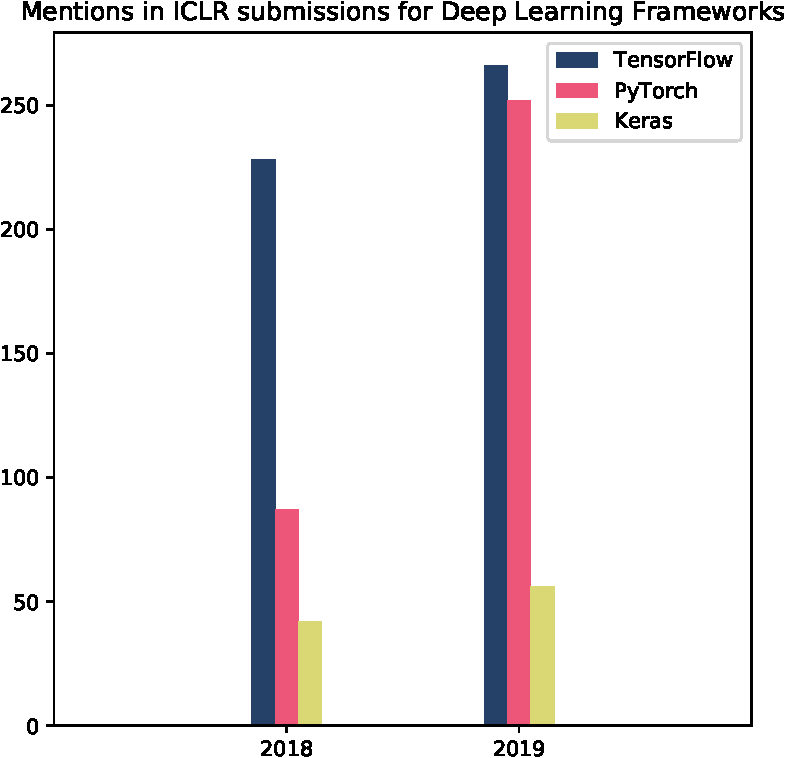
\includegraphics[max width=\textwidth]{gfx/diagrams/framework_popularity/popularity.pdf}
        \caption[Changes in popularity of different deep learning libraries in
        research]{Changes in popularity of different deep learning libraries in
            research. Data was collected by keyword search over ICLR submissions
            (\href{http://search.iclr2019.smerity.com/search/}{http://search.iclr2019.smerity.com/search};
        analogously for 2018)}\label{fig:popularity}
    }
\end{figure}

\hypertarget{sec:pubsub}{%
\section{Publisher-Subscriber}\label{sec:pubsub}}

The Publisher-Subscriber pattern (for a detailed overview see
\cite{eugster2003}) is a pattern for distributed computation in which publishers
publish messages either directly to any subscribers which have registered
interest in them, or to a central authority orchestrating the exchange. Messages
are generally associated with one or more topics and subscribers register
interest in receiving messages on one or more topics.

The compontens are very loosely coupled; the subscribers need not even
be aware of the publishers at all, and the publishers' only interaction
with their subscribers is relaying messages through a uniform interface
or through an optional server. A graphical schema of one possible
incarnation of this pattern is shown in \cref{fig:pubsub}.

\begin{figure}
    \hypertarget{fig:pubsub}{%
        \centering
        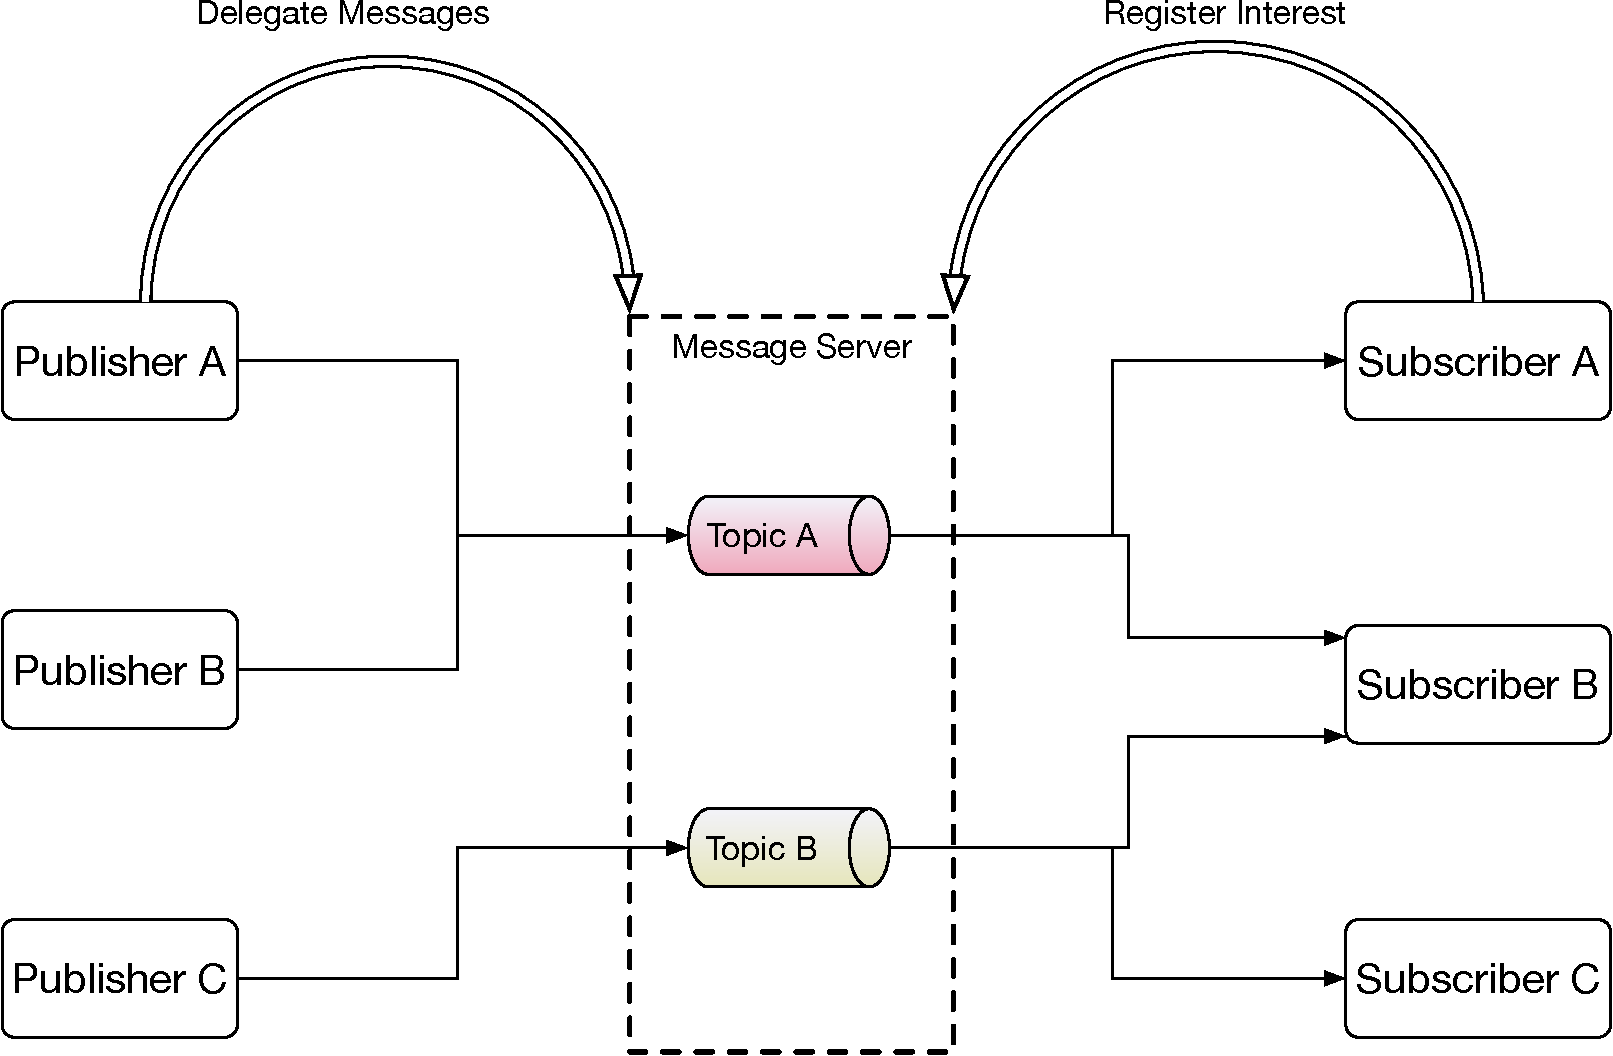
\includegraphics[max width=\textwidth]{gfx/diagrams/architecture_diagrams/pubsub.pdf}
        \caption{One possible implementation of the Publisher-Subscriber pattern.}\label{fig:pubsub}
    }
\end{figure}

This project is not distributed, but can benefit from the loose coupling
in another way: Subscribers can be defined in terms of the kind of
messages they need to compute their metric, without knowing anything
about where the messages are coming from. Concretely, as long as the
appropriate data is emitted from the training process, subscribers can
work without modifications with any possible model.

Since real-world neural networks are trained on the GPU, and
communication between host and GPU memory is already expensive, making this
library truly distributed is not an objective. However, the design will
simplify asynchronous computation of metrics in the future. The Python
language does not support true multithreading\footnote{The
    \texttt{multiprocessing} module allows for truly
    asynchronous computation and communication, but the
    inter-process-communication is more expensive than memory shared
between threads.}, but since the expensive part of the work is running
on the GPU while the host code is waiting, metric computation could
happen asynchronously on the GPU as well while the expensive forward or
backward passes through the network are running. This is not currently
implemented but can be added later, if more computationally demanding
metrics are to be explored.

In the context of neural network training, there is only one source of
information and hence only one publisher. Nevertheless, a message server is
introduced to segregate responsibilities. The singular publisher extracts data from the
training model, passes it on to the server which also accepts subscriber
registrations and relays messages appropriately.

\hypertarget{overview-of-the-library}{%
\section{Overview of the library}\label{overview-of-the-library}}

The software is structured into several packages. The root package is
\texttt{ikkuna} which encapsulates all core
functionality. All other packages and modules contain utilites
implemented for this work specifically, but will generally not be
relevant to other users. A survey of these tools will be given in
\cref{sec:other-tools}.

The root package diagram is shown in \cref{fig:pack-diag-ikkuna}

\begin{figure}
    \hypertarget{fig:pack-diag-ikkuna}{%
        \centering
        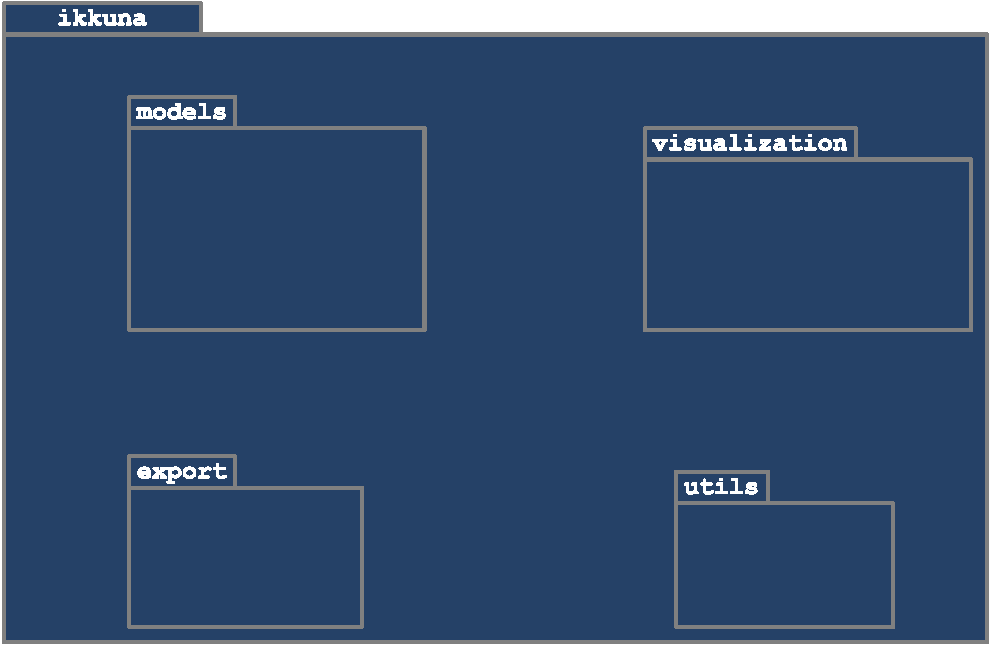
\includegraphics[max width=.7\textwidth]{gfx/diagrams/class_diagrams/ikkuna_package_diagram.pdf}
        \caption{\texttt{ikkuna} package diagram}\label{fig:pack-diag-ikkuna}
    }
\end{figure}

The \texttt{models} (see \cref{sec:pack-models})
subpackage contains a few exemplary neural network definitions which are
wired up with the library and can thus be used to showcase the library's
functionality. The \texttt{utils} (see
\cref{sec:pack-utils}) subpackage contains miscellaneous utility classes
and functions used throughout the core library. Lastly, the
\texttt{visulization} subpackage
(\cref{sec:pack-visualization}) contains the plotting functionality to
actually show the metrics computed during the training process.

The most important bits of the software live in the
\texttt{export} subpackage (\cref{sec:pack-export}). It
implements the Publisher-Subscriber pattern. Extracting data from the
training process, defining subscriber functionality and messages used
for communication is done here.

\hypertarget{sec:pack-export}{%
\subsection{The \texttt{export} subpackage}\label{sec:pack-export}}

The \texttt{export} subpackage contains the core part
of the library, i.e.~it provides the classes that handle discovering the
structure of the neural network model, attaching the appropriate
callbacks and intercepting method calls on the model so the library is
informed about everything entering and exiting the model and its
individual layers. It also contains the definition for the subscriber
API, i.e.~the messages that subscribers can receive, synchronisation
facilities when multiple topics are needed by a subscriber, as well as
the subscriber class interface. The package diagram is displayed in
\cref{fig:pack-diag-export}.

The package comprises three subpackages or modules listed in
\cref{tbl:ikkuna.export}

\begin{table}
    \caption{\texttt{ikkuna.export} functionalities}
    \label{tbl:ikkuna.export}
    \begin{tabularx}{\textwidth}{lX}
        \toprule
        Name                & Function\tabularnewline
        \midrule
        \texttt{export}     & Publish data from an arbitrary model and send messages to registered subscribers\tabularnewline
        \texttt{messages}   & Define message interface; i.e.~what topics exist and which information a message must contain\tabularnewline
        \texttt{subscriber} & Define the base class for metric subscribers\tabularnewline
        \bottomrule
    \end{tabularx}
\end{table}

\subsubsection*{The \texttt{ikkuna.export} subpackage}

\begin{figure}
    \hypertarget{fig:pack-diag-export}{%
        \centering
        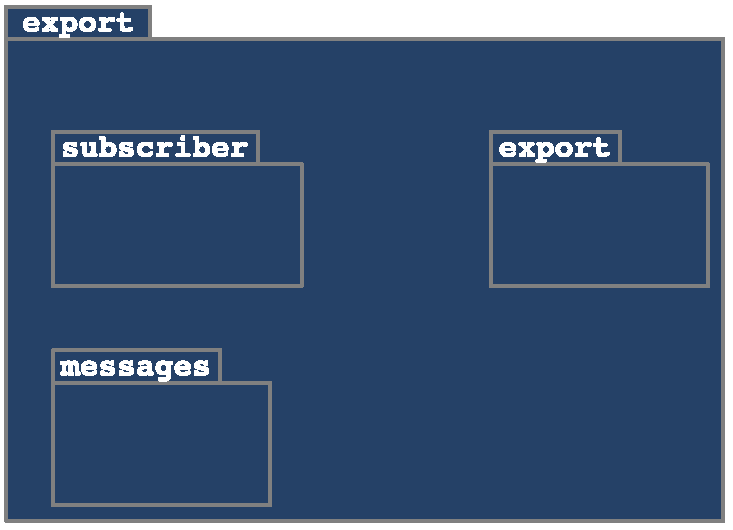
\includegraphics[max width=.7\textwidth]{gfx/diagrams/class_diagrams/export_package_diagram.pdf}
        \caption{\texttt{ikkuna.export} package diagram}\label{fig:pack-diag-export}
    }
\end{figure}

In in slight deviation from the Publisher-Subscriber framework as displayed in
\cref{fig:pubsub}, the \texttt{export.Exporter} class
(\cref{fig:class-diag-exporter}) is the sole publisher of data. There is only one
source of data during training, so it is unnecessary to accomodate multiple
publishers. The \texttt{Exporter} is informed of the model with its methods
\lstinline{set_model()} and \lstinline{set_loss()}, the latter of which is only
necessary if metrics which rely on training labels should be displayed.  It can
accept a filter list of classes which are to be included when discovering the
modules in the model. For instance, it could be desirable to only observe layers
which have weights and biases associated with them, not e.g.~normalisation or
reshaping layers. The \texttt{Exporter} then traverses the model (which is
really just a tree structure of modules) and adds to each a callback invoked
when input enters the layer -- in order to retrieve activations -- and when
gradients are computed for the layer outputs. The callbacks also use cached
weights -- if present -- in order to publish updates to the weights.
Furthermore, it replaces a few of the model's methods with closure wrappers so
it can

\begin{itemize}
    \item
        be notified when the model is set to training or testing mode (this
        switch disables or enables layers which only make sense during one of
        the phases\footnote{There are two built-in layers this applies to. One
            is the batch normalisation layer. It normalises the output of the
            previous layer with the mean and variance over the entire batch of
            data -- optionally with running means and variances over the
            previousprevious training steps. The variance is not defined for
            single data point enters the layer, as could be the case during
            inference/testing time. The second case is the dropout layer, which
            randomly zeroes out a percentage of the previous layer's
            activations. This is used during training to prevent subsequent
            units from becoming correlated with a fixed set of units in the
            previous layer, instead of picking up patterns invariant of where in
            the input they occur. During inference time, this is turned off to
            make full use of the trained
        layers.})
    \item
        increase its own step counter automatically when a new batch is seen
    \item
        add a parameter to the model's \lstinline{forward()} method -- called by
        the runtime when data is propagated through the model -- which can be
        used be subscribers to temporarily turn off training mode and have it
        revert automatically. This is useful for subscribers which need to
        evaluate the model (i.e.~feed data through it), but do not want to
        generate new messages for this occasion.
    \item
        intercept labels passed to the loss function during training and
        publish them as messages so the user need not concern himself with
        this task
    \item
        intercept the final output of the network. This could be realised
        alternatively by identifying the last module in the network.
\end{itemize}

At every time step (training batch), the \texttt{Exporter} publishes the
following information on to the message bus (see \cref{fig:messages_class_diag}):

\begin{itemize}
    \item
        gradients for each module
    \item
        activations for each module
    \item
        weights and biases for each module that has these properties
        (e.g.~convolutional or fully-connected layers)
    \item
        updates to the weights and biases from the last step to the current
        one, provided the module has these properties
    \item
        Training labels used for the parameter updates. This requires that the
        \texttt{Exporter} be informed of the loss function object with
        \lstinline{set_loss()}.
    \item
        The batch of input data passed to the network at the current training step
    \item
        The final output of the network for the current batch of training data.
        This is simply the tensor of activations from the last layer and is thus
        technically duplicated since activations are published anyway. The
        reason is that some subscribers may only be interested in the network
        predictions and it is unnecesary to determine automatically the last
        layer in the network as the loss function has automatic access to
        the activations and must be tracked anyway for the training labels
\end{itemize}

Further messages are published only at certain points in the training process

\begin{itemize}
    \item
        When a batch starts or ends, a message with the current batch index is published
    \item
        When an epoch starts or ends, a message with the current batch index is
        published. This requires the \texttt{Exporter} be notified with
        \lstinline{epoch_finished()} by the user, since it is impossible to
        determine when an epoch is over from inside the model.
\end{itemize}

\subsubsection*{The \texttt{ikkuna.export.messages} submodule}

This submodule contains definitions of all permissible messages kinds, message
classes and a collection class for message objects. An overview of the classes
defined in this module is shown in \cref{fig:messages_class_diag}.

\begin{figure}
    \centering
    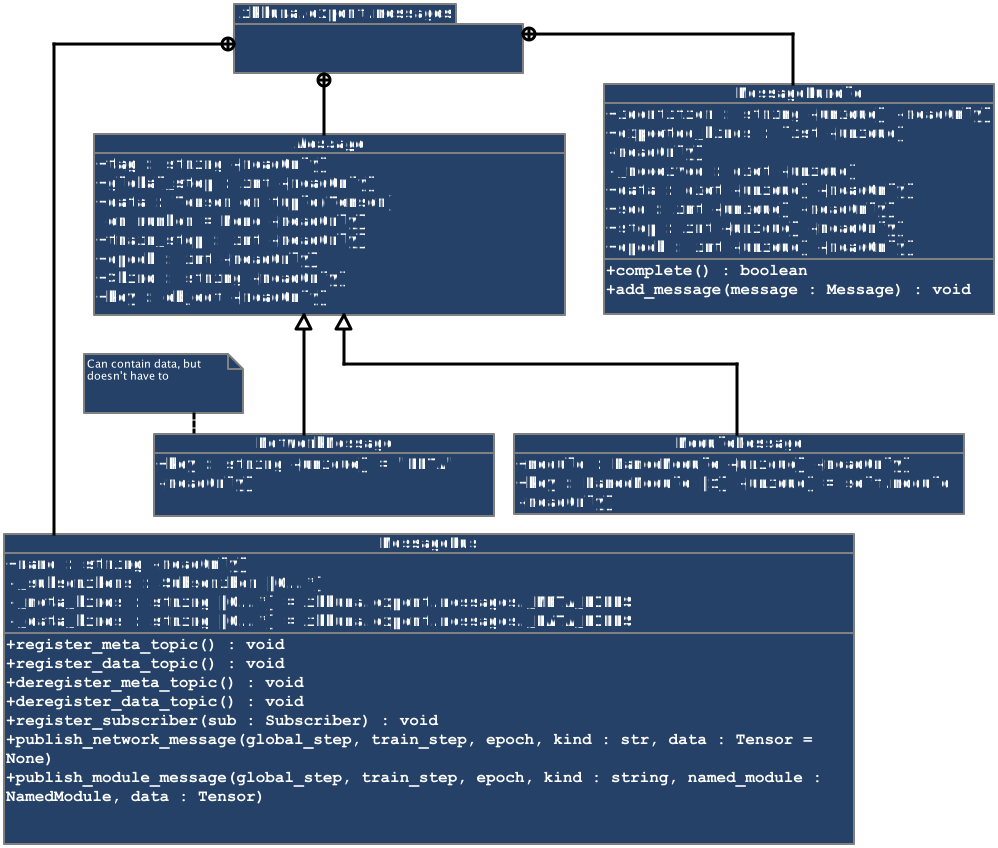
\includegraphics[width=\textwidth]{{gfx/diagrams/class_diagrams/ikkuna.export.messages}.pdf}
    \caption{Classes in the \texttt{ikkuna.export.messages} submodule}
    \label{fig:messages_class_diag}
\end{figure}

Messages are of one of two types: They are either directly tied to a layer in
the network and are thus published for each layer, or they contain information
for the current training step applying to the entire network. In that case, they
appear only once per training step, not once per layer. The meta-messages can
carry tensor data (e.g.~input data or labels), but need not to
(e.g.~notifications about a starting or ending epoch). All message kinds are
summarised in \cref{tbl:messages}.

Messages can be assembled into bundles if a subscribers wants to subscribe
several topics at once. The \texttt{MessageBundle} class performs all necessary
error checking to ensure consistency of the contained messages.

The message server from \cref{fig:pubsub} is implemented by the
\texttt{MessageBus}  class which publishers publish messages onto, accepts
subscriber registrations, and maintains the lists of known topics. Each
subscriber may in turn announce one or more new topics which can then be
subscribed to by others. This is useful since it allows chaining of subscribers
in order to realise arbitrary post-processing of computed metrics.

\begin{table}
    \centering
    \caption{Subscribable message kinds}
    \label{tbl:messages}
    \begin{tabularx}{\textwidth}{llX}
        \toprule
        \rowcolor{verylightblue}\multicolumn{3}{c}{Meta topics} \tabularnewline
        \midrule
        Identifier                     & Frequency                & Description \tabularnewline
        \midrule
        {\lstinline!batch_started!}    & Once every batch         & \tabularnewline
        {\lstinline!batch_finished!}   & \ditto                   & \tabularnewline
        {\lstinline!epoch_started!}    & Once every epoch         & \tabularnewline
        {\lstinline!epoch_finished!}   & \ditto                   & \tabularnewline
        {\lstinline!input_data!}       & Once every batch         & \tabularnewline
        {\lstinline!input_labels!}     & \ditto                   & \tabularnewline
        {\lstinline!network_output!}   & \ditto                   & Activations of the last layer \tabularnewline
        \bottomrule
        \rowcolor{verylightblue}\multicolumn{3}{c}{Data topics} \tabularnewline
        \midrule
        Identifier                     & Frequency                & Description \tabularnewline
        \midrule
        {\lstinline!weights!}          & Once per layer per batch & Gradients of loss function w.r.t. layer weight matrix \tabularnewline
        {\lstinline!weight_gradients!} & \ditto                   & \tabularnewline
        {\lstinline!weight_updates!}   & \ditto                   & \tabularnewline
        {\lstinline!biases!}           & \ditto                   & Gradients of loss function w.r.t. layer bias matrix \tabularnewline
        {\lstinline!bias_gradients!}   & \ditto                   & \tabularnewline
        {\lstinline!bias_updates!}     & \ditto                   & \tabularnewline
        {\lstinline!activations!}      & \ditto                   & \tabularnewline
        {\lstinline!layer_gradients!}  & \ditto                   & Gradients of loss function w.r.t. layer output \tabularnewline
        \bottomrule
    \end{tabularx}
\end{table}

\begin{figure}
    \hypertarget{fig:class-diag-exporter}{%
        \centering
        \includegraphics[max width=.8\textwidth]{gfx/diagrams/class_diagrams/{ikkuna.export.Exporter}.pdf}
        \caption{\texttt{ikkuna.export.Exporter} class diagram}\label{fig:class-diag-exporter}
    }
\end{figure}

\subsubsection*{The \texttt{ikkuna.export.subscriber} subpackage}

The third subpackage contained in the \texttt{ikkuna.export} package defines the
subscriber part of the Publisher-Subscriber pattern. The diagram of the defined
classes is shown in \cref{fig:class-diag-subscriber}. The \texttt{Subscriber}
base class is rudimentary and mandates only the implementation of the metric
computation by subclasses. In the simplest case, a subscribers is interested in
only one topic and therefore is coupled to a simple \texttt{Subscription}
object, which handles bookkeeping tasks such as subsampling the messaage stream,
routing only relevant messages to the subscriber and counting the received messages.

More generally however, a subscriber may want to receive several pieces of
information for each layer in each time step (i.e.~for computing the ratio
between weight updates and weights). Since the order of messages is not
guaranteed, the desired messages are unlikely to occur one after the other;
instead the topics must be synchronised. A \texttt{SynchronizedSubscription}
buffers messages of the relevant topics until all requested kinds have been
received for the current training step, before releasing them to the subscriber.

A subscriber can thus receive a single message or a bundle of messages.

The library comes with a few subscribers already installed (they are themselves
plugins, see \cref{plugin-infrastructure}). Details are given in
\cref{tbl:subscribers}

\begin{figure}
    \centering
    \includegraphics[width=\linewidth]{gfx/diagrams/class_diagrams/{ikkuna.export.subscriber}.pdf}
    \caption{Classes defined in \texttt{ikkuna.export.subscriber}}
    \label{fig:class-diag-subscriber}
\end{figure}

\begin{table}
    \centering
    \caption{Pre-packaged subscriber subclasses}
    \label{tbl:subscribers}
    \begin{tabularx}{\textwidth}{lX}
        \toprule
        Name                             & Functionality                                                                                                                                                         \tabularnewline
        \midrule
        \texttt{MeanSubscriber}          & Computes the mean $\mu = \frac{1}{n}\sum_{i=1}^n w_i$ of a tensor                                                                                                     \tabularnewline
        \texttt{VarianceSubscriber}      & Computes the variance $\sum_{i=1}^n (w_i - \mu)^2$ for a tensor                                                                                                       \tabularnewline
        \texttt{SumSubscriber}           & Computes the sum $\sum_{i=1}^n w_i$ of a tensor                                                                                                                       \tabularnewline
        \texttt{NormSubscriber}          & Computes the $p$-Norm $\sqrt[p]{\sum_{i=1}^n w_i^p}$                                                                                                                  \tabularnewline
        \texttt{RatioSubscriber}         & Computes the average ratio $\frac{1}{n}\sum_{i=1}^n \frac{a_i}{b_i}$ of two tensors, disregarding NaN values                                                          \tabularnewline
        \texttt{HistogramSubscriber}     & Computes the histogram of a given tensor. This is computationally heavy.                                                                                              \tabularnewline
        \texttt{SpectralNormSubscriber}  & Computes the spectral norm (largest signular value) $\max_{\mathbf{h}:\mathbf{h}\neq 0} \frac{\left||A\mathbf{h}\right||_2}{\left||\mathbf{h}\right||_2}$ of a tensor \tabularnewline
        \texttt{TestAccuracySubscriber}  & Computes the ratio of correctly classified examples to total examples over the test set                                                                               \tabularnewline
        \texttt{TrainAccuracySubscriber} & Computes the ratio of correctly classified examples to total examples over current batch of training data                                                             \tabularnewline
        \bottomrule
    \end{tabularx}
\end{table}

\hypertarget{sec:pack-models}{%
\subsection{The \texttt{models} subpackage}\label{sec:pack-models}}

\begin{figure}
    \hypertarget{fig:pack-diag-models}{%
        \centering
        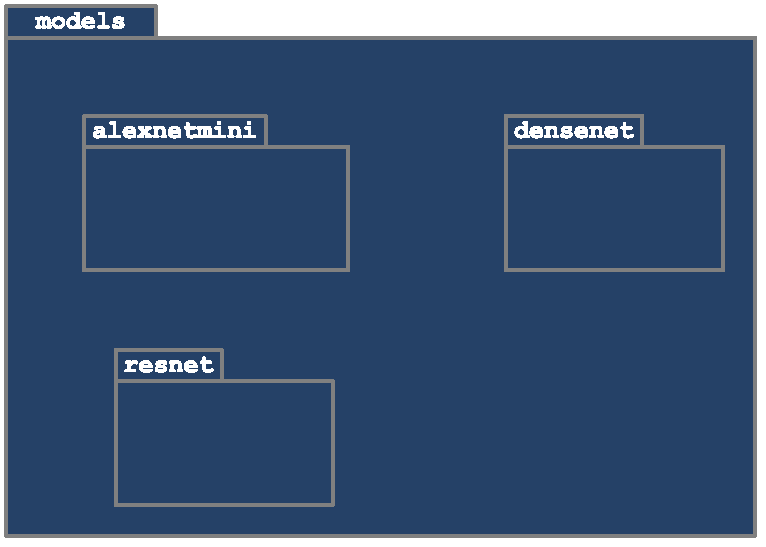
\includegraphics[max width=.7\textwidth]{gfx/diagrams/class_diagrams/models_package_diagram.pdf}
        \caption{\texttt{ikkuna.models} package diagram}\label{fig:pack-diag-models}
    }
\end{figure}

This package shown in \cref{fig:pack-diag-models} contains model
definitions for demonstration purposes and for experimentation. Three
architectures are currently implemented:

\begin{enumerate}
    \item
        A minified version of AlexNet, since the original architecture
        requires larger images \citep{krizhevsky2012imagenet}. The
        code is adapted from
        \url{https://github.com/sukilau/Ziff-deep-learning/blob/master/3-CIFAR10-lrate/CIFAR10-lrate.ipynb}.
    \item
        DenseNet \citep{huang2017densely}. The implementation is basically the
        one from \citep{pleiss2017memory}\footnote{At the time of writing, the
            implementation is available here:
            \url{https://github.com/gpleiss/efficient_densenet_pytorch/blob/master/models/densenet.py}.
            The licensing is unclear as the author references the original
            BSD-licensed implementation at
            \url{https://github.com/pytorch/vision/blob/master/torchvision/models/densenet.py}
            which was licensed by PyTorch core contributor Soumith Chintala.
            However, the code does not reproduce the BSD license text and can
            thus only be inspired by the original but cannot contain any of the
        code verbatim. It would require careful examination in order to
    determine whether this is the case.} with minor modifications
    \item
        ResNet \citep{he2016deep}. This implementation comes from
        GitHub user liukang\footnote{The implementation is MIT-licensed.
        \url{https://github.com/kuangliu/pytorch-cifar/blob/master/models/resnet.py}}
        and can handle CIFAR10-sized images of 32 pixels per side, as opposed
        to most implementaions that are geared towards ImageNet examples which
        are much larger.
\end{enumerate}

All models are modified such that their training can be supervised by
the library.

\hypertarget{sec:pack-utils}{%
\subsection{The \texttt{utils} subpackage}\label{sec:pack-utils}}

As shown in \cref{fig:pack-diag-utils}, this package defines classes for
traversing a model into a hierarchical tree of layers (called \emph{modules} in
PyTorch lingo), structures for adding information to PyTorch's \texttt{Module}
class, and a set of miscellaneous functions for

\begin{enumerate}
    \item
        Seeding random number generators to make experiments reproducible (see
        \cref{ch:appendixB})
    \item
        Creating instances of weight optimizers by named
    \item
        Initialize the weights of any model
    \item
        Loading datasets
\end{enumerate}

\begin{figure}
    \hypertarget{fig:pack-diag-utils}{%
        \centering
        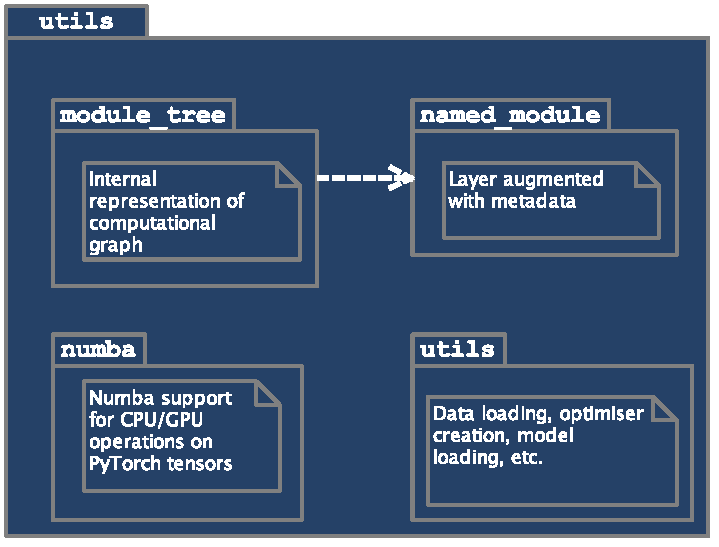
\includegraphics[max width=.7\textwidth]{gfx/diagrams/class_diagrams/utils_package_diagram.pdf}
        \caption{\texttt{ikkuna.utils} package diagram}\label{fig:pack-diag-utils}
    }
\end{figure}

Additionally, it contains the \texttt{numba} module
which is inteded to allow interoperability with the Numba
library\footnote{\url{https://numba.pydata.org/}. Numba is a library for
    transforming high-level Python code into performant compiled code and
    for allowing to use the CUDA library from Python with Python arrays.
    This enables performance improvements for numeric calculations, but
    there is only a limited set of higher-level functions implemented on
GPU arrays.}. While currently not used due to the incomplete nature of
the Numba GPU array interface, it could enable leveraging Numba in the
future without transferring data to the CPU. The core function was later
obsoleted by an addition to the PyTorch library\footnote{The main contribution
of the submodule was to make PyTorch tensors accesible to Numba by
monkey-patching the \lstinline{__cuda_array_interface__} property. This has since
been added via pull request \#11984 to the PyTorch repository.}.

\hypertarget{sec:pack-visualization}{%
\subsection{The \texttt{visualization} subpackage}\label{sec:pack-visualization}}

This package contains only a single module:
\texttt{backend}. It defines the classes shown in
\cref{fig:class-diag-backend}. The module serves as an abstraction over
plotting libraries so that metrics need not concern themselves with how
to actually show the data.

A given metric will compute its value and dispatch it to its
visualization backend, which can currently accept scalar and histogram
data. The metric class itself need not care about how it is going to be
displayed.

\begin{figure}
    \hypertarget{fig:class-diag-backend}{%
        \centering
        \includegraphics[max width=\textwidth]{gfx/diagrams/class_diagrams/{ikkuna.visualization}.pdf}
        \caption{Class diagram for classes in \texttt{ikkuna.visualization}}\label{fig:class-diag-backend}
    }
\end{figure}

For running the library locally, a \texttt{matplotlib}-based backend has been
implemented.  Plotting routines from this library open a window directly on the
system executing the software. In practice however, deep learning code will be
executed remotely on a server with adequate compute capability and the
programmer connected via SSH. While it is possible to have remote windows show
up locally on Linux-based systems by use of X11-Forwarding, this is generally
slow and not useful for interactivity. An example is shown in
\cref{fig:example_mpl} To remedy this issue, a plotting backend for TensorBoard
(see \cref{sec:existing-apps}) is also provided. The plotting data is generated
and processed on the remote system, but served over the web so it can be viewed
and interacted with locally (provided the network is configured so that the
server responds to HTTP requests). An example is shown in \cref{fig:example_tb}.

\begin{figure}
    \hypertarget{fig:example_mpl}{%
        \centering
        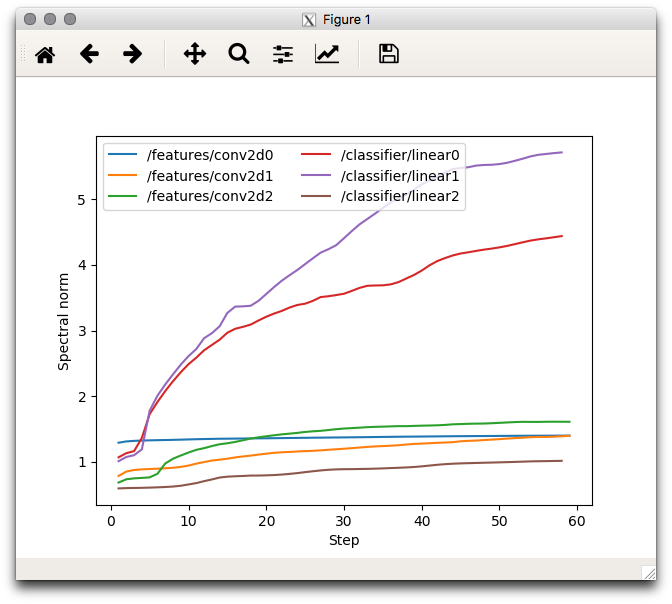
\includegraphics[max width=\textwidth]{gfx/diagrams/software_screens/example_mpl.png}
        \caption{Exemplary view of a matplotlib figure forwarded over SSH}\label{fig:example_mpl}
    }
\end{figure}

\begin{figure}
    \hypertarget{fig:example_tb}{%
        \centering
        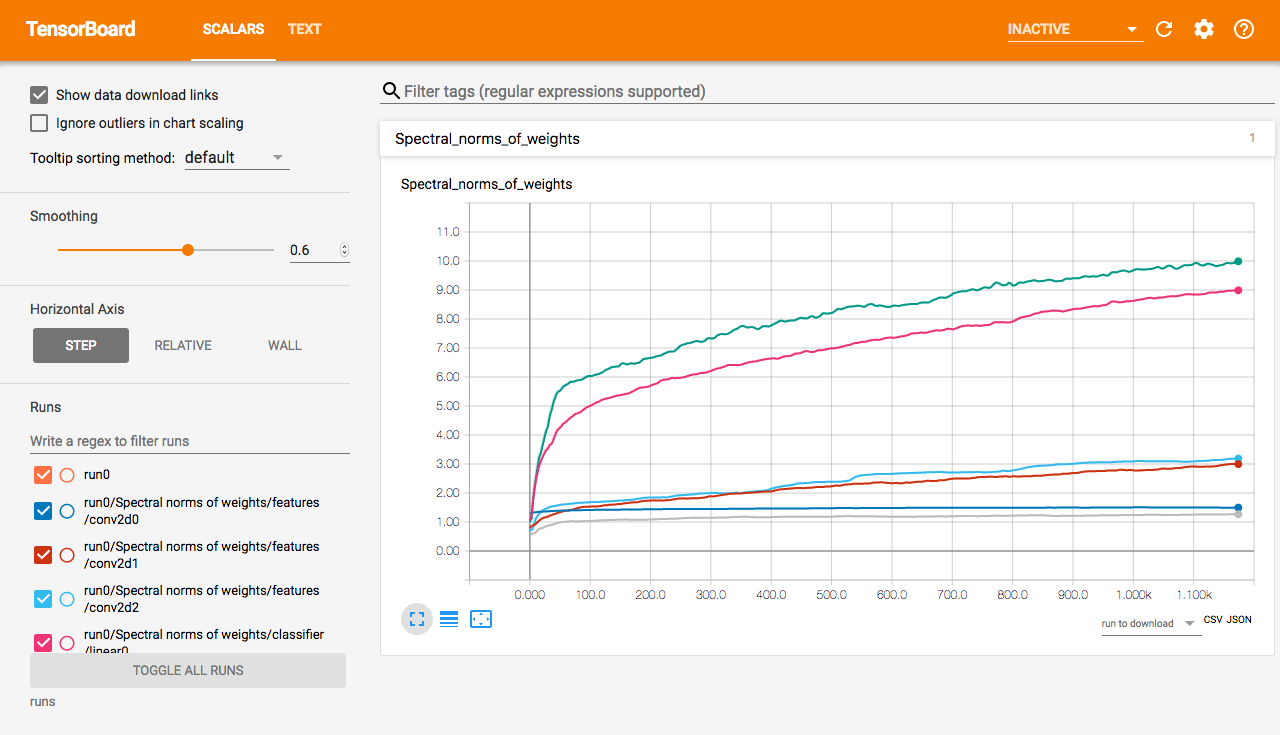
\includegraphics[width=\textwidth]{gfx/diagrams/software_screens/example_tb.png}
        \caption{Exemplary view of a TensorBoard session}\label{fig:example_tb}
    }
\end{figure}

\hypertarget{sec:other-tools}{%
\subsection{Miscellaneous tools}\label{sec:other-tools}}

There are a few modules which simplify development with the library but are not
part of the distribution obtained from PyPi or by running the setup script.

The \texttt{train} package defines a \texttt{Trainer} class which encapsulates
all the logic and parameters needed to train a neural network on one of the
datasets provided with PyTorch. The class's capabilities include the following

\begin{itemize}
    \item
        Look up model and dataset by name
    \item
        Bundle all hyperparameters
    \item
        hook the \texttt{Exporter} into the model for
        publishing data
    \item
        configure the optimisation algorithm to use for training
    \item
        train the model for one batch
\end{itemize}

The \texttt{Trainer} class is used in the main script (\texttt{main.py}), which
serves as a command line interface to the library while developing. When trying
out the library, it can also be used as an initial starting point.

\begin{table}
    \caption{Named arguments to \texttt{main.py}}
    \begin{tabularx}{\linewidth}{lX}
        \toprule
        Parameter                                   & Explanation\tabularnewline
        \midrule
        \lstinline{-m}, \lstinline{--model}         & Model class to train\tabularnewline
        \lstinline{-d}, \lstinline{--dataset}       & Dataset to train on. Possible choices: \lstinline{MNIST}, \lstinline{FashionMNIST}, \lstinline{CIFAR10}, \lstinline{CIFAR100}\tabularnewline
        \lstinline{-b}, \lstinline{--batch-size}    & Default: 128\tabularnewline
        \lstinline{-e}, \lstinline{--epochs}        & Default: 10\tabularnewline
        \lstinline{-o}, \lstinline{--optimizer}     & Optimizer to use. Default: \lstinline{Adam}\tabularnewline
        \lstinline{-a}, \lstinline{--ratio-average} & Number of ratios to average for stability (currently unused). Default: 10\tabularnewline
        \lstinline{-s}, \lstinline{--subsample}     & Number of batches to ignore between updates. Default: \lstinline{1}\tabularnewline
        \lstinline{-v}, \lstinline{--visualisation} & Visualisation backend to use. Possible choices: \lstinline{tb}, \lstinline{mpl}. Default: \lstinline{tb}\tabularnewline
        \lstinline{-V}, \lstinline{--verbose}       & Print training progress. Default: \lstinline{False}\tabularnewline
        \lstinline{--spectral-norm}                 & Use spectral norm subscriber on weights. Default: \lstinline{False}\tabularnewline
        \lstinline{--histogram}                     & Use histogram subscriber(s)\tabularnewline
        \lstinline{--ratio}                         & Use ratio subscriber(s)\tabularnewline
        \lstinline{--test-accuracy}                 & Use test set accuracy subscriber. Default: \lstinline{False}\tabularnewline
        \lstinline{--train-accuracy}                & Use train accuracy subscriber. Default: \lstinline{False}\tabularnewline
        \lstinline{--depth}                         & Depth to which to add modules.  Default: \lstinline{-1}\tabularnewline
        \bottomrule
    \end{tabularx}
\end{table}

The library can be installed to the local Python environment by use of the
provided setuptools script (\texttt{setup.py}). It can also be downloaded from
the \href{https://pypi.org/}{Python Package Index} by use of the package manager
\texttt{pip}:
\begin{lstlisting}[language=Python]
pip install ikkuna
\end{lstlisting}

\hypertarget{plugin-infrastructure}{%
\subsection{Plugin Infrastructure}\label{plugin-infrastructure}}

Among the main selling points of this library is the provision to add new
metrics as plugins and reuse them system-wide for all architectures. Plugins in
Python projects can be enabled through appropriate use of the
\texttt{setuptools} library. During the setup process for installing the
library, entry points are defined by the library which can be used by plugins to
announce themselves. Ikkuna provides the
\lstinline[language=Python,breaklines=false]{'ikkuna.export.subscriber'} entry
point. For registering a plugin, the author must simply use that entry point to
make a plugin available either through the package it is defined in, or through
the \lstinline{ikkune.export.subscriber} namespace. For illustration,
\cref{lst:plugin} shows how to setup a \texttt{setup.py} setuptools file. The
plugin can be installed like any other Python package with
\begin{lstlisting}[language=Python]
python setup.py install
\end{lstlisting}
which will install all required dependencies inside the current environment. The
PyTorch library must be installed manually since the binaray distribution is too
old at the time of writing. Detailed instructions can be found in the user guide
which is part of the documentation.

\begin{lstlisting}[label=lst:plugin, language=Python, caption=Sample setup script for subscriber plugins]
#!/usr/bin/env python

from distutils.core import setup
import setuptools

setup(name='<your package name>',
    version='<version>',
    description='<description>',
    author='<your name',
    author_email='<your email>',
    packages=['<package name>'],
    # ... any other args
    entry_points={
        'ikkuna.export.subscriber': [
            'YourSubscriber = module.file:YourSubscriber',
        ]
    })
\end{lstlisting}

\subsection{Documentation}\label{doc}

The entire codebase is liberally documented using the Sphinx documentation
processor\footnote{\url{http://www.sphinx-doc.org/}}. The documentation contains
further documents with a detailed user guide, installation instructions. Sphinx
allows generating documentation in many formats from the same source, most
usefully HTML and PDF. At the time of writing, the HTML documentation and API
reference is hosted at \url{https://peltarion.github.io/ai_ikkuna/}.

\section{Business Case for the Library}\label{business-case}

This work is done in cooperation with Peltarion
AB\footnote{\url{http://www.peltarion.com/}}, a software company based in
Stockholm, Sweden. Peltarion's stated mission is to

\begin{quote}
    [provide] an
    operational AI platform for producing real-world AI applications at scale and at
    speed.
\end{quote}

The Peltarion platform is a web-based deep learning platform with which users
can upload, preprocess and modify datasets, create deep neural architectures
without having to write code and track performance of each model and dataset
version through experiment versioning. Trained models can be directly deployed
as a webservice.

The modeling interface presented to the user is shown in \cref{fig:platform}

\begin{figure}
    \centering
    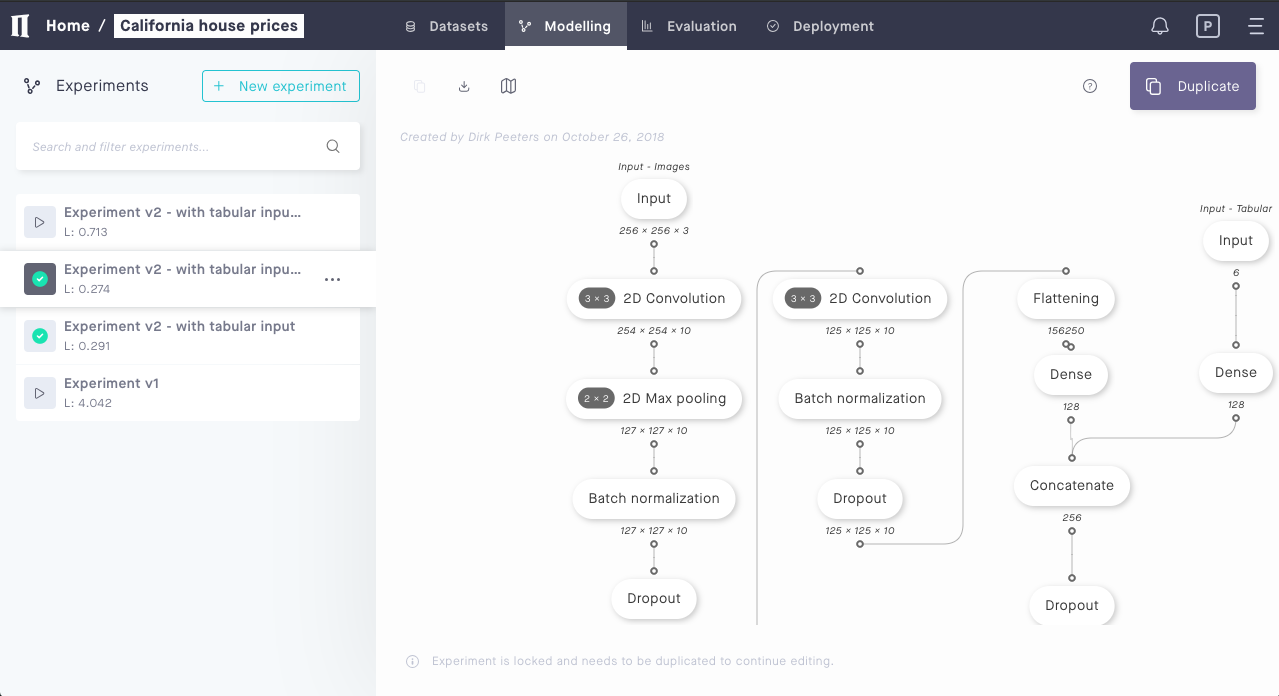
\includegraphics[width=\textwidth]{gfx/diagrams/software_screens/peltarion_platform.png}
    \caption{The Peltarion platform modeling screen}
    \label{fig:platform}
\end{figure}

While the product in question is code-free for the user, it is powered by a deep
learning framework on the server side. The business proposition made by
Peltarion is to make training deep neural networks more affordable, which the
company wants to realise through savings in development time from problem
statement to model deployment. As outlined in \cref{sec:motivation}, development
of state-of-the art deep learning applications requires both expertise and
education as well as experience. Since experts in any discipline are rare and
expensive, lowering the cost in this area requires simplifying the process of
creating deep learning solutions. A code-free platform is one way to accomplish
this and make deep learning more accesible to users and companies without the
previously required expertise in research and engineering.

This ties into this objective in two ways. Firstly, by providing an API against
which training metrics can easily be implemented and served to arbitrary
backends, engineering effort for metric features of the platform is reduced. For
this work, plotting backends have been implemented, but the decoupled compontent
architecture of the \texttt{ikkuna} library was chosen precisely to enable
arbitrary data sinks for the computed metrics, for instance a web service or a
database which is accessed by the Peltarion platform to display metrics to the
user. The engineering team at Peltarion could make use of this library to handle
metric logging on arbitrary models created by the platform's users without
having to resort to code generation during translation of the abstract model
definition created in the browser to the model implementation in the backend.

Secondly, the library -- or the ideas prototyped therein -- will be helpful in
providing feedback to the user about the state of their experiment. Since the
platform is at least partially aimed at non-experts, even well-known and simple
metrics can be of great help in avoiding common pitfalls in model training. This
directly reduces the opaqueness of the training process to the non-expert user,
reducing time wasted on fruitless experiments and increasing confidences in the
product.

It should be stressed, however, that the software implemented for this thesis is
free and open-source and not owned or licensed by Peltarion AB.


\appendix

\chapter{Appendix A --- Open Source Acknowledgments}
\label{ch:appendixA}

The following presents a non-exhaustive list of open source tools used in
creating the software, experiments and this document:
\begin{enumerate}
    \item \LaTeX{} for typesetting this document \citep{lamport}. This includes contributions by
        the creators of all the packages which make up the typesetting
        environment.
    \item The various GNU and thrid-party command line tools (\texttt{grep}, \texttt{parallel}
        \citep{tange_ole_2018_1146014}, \texttt{latexmk} etc.)
    \item The Ubuntu operating system and the Linux kernel
        \citep{torvalds2008linux} providing the
        computational environment for the experiments conducted for this work,
        alongside the GNU compiler toolchain for compiling software
        for the system
    \item The TMUX and SSH tools for connecting to the system running the
        experiments
    \item The PyTorch \citep{paszke2017automatic}, Numpy, TensorBoard and
        Matplotlib libraries \citep{scipy} used for the
        software, based all on the Python programming language and standard
        library.
    \item The Sacred \citep{sacred}, MongoDB and Pymongo libraries used for logging experiments
        to a database for later visualisation
    \item The Vim editor and associated plugin ecosystem employed for creating
        all documents, be it code or documentation
    \item The Git source control management tool which was used to version both
        software and documentation artifacts
\end{enumerate}


\bibliography{Bibliography}{}
\addcontentsline{toc}{chapter}{\scshape Bibliography}


\chapter*{Acknowledgments}

I wish to acknowledge the contributions of many people who---directly or
indirectly---supported this work.

I thank Justin Shenk for providing the introduction to the Peltarion team and
his generosity and company while travelling with me and---along with
Veine Haglund---hosting me for my visits to Stockholm.

I am also grateful to Anders Arpteg who has been a constant source of support
and advice, for his willingness to let me work on my own terms on what I saw fit.

Thanks as well to Justin, Anders and Mikael Huss for feedback on thesis drafts.

I owe further thanks to Oliver Vornberger who agreed to act as first
examiner for this thesis, instead of enjoying retirement, and Ulf Krumnack
for acting as co-examiner and providing feedback on this work.

I thank the entire team at Peltarion AB for creating a welcoming and very
entertaining environment for working on this thesis and providing computational
resources making this work possible at all.  Also for the ice cream.

Lastly, I wish to acknowledge the countless unnamed developers of the myriads of
open source tools that form the bedrock of any productive scientific endeavour.
A highly non-exhaustive list of software used during the creation of this thesis can be found in
\cref{ch:appendixA}.


\chapter*{Declaration of Authorship}

I hereby certify that the work presented here is---to the best of my knowledge
and belief---original and the result of my own investigations, except as
acknowledged, and has not been submitted, either in part or whole, for a degree
at this or any other university.

\vspace{2cm}

\noindent\rule{5cm}{1pt}

\noindent Rasmus Diederichsen \hfill{} Osnabrück, \today


\end{document}
